\chapter{Sina Weibo et le milieu numerique en Chine} 

Ce premier chapitre présenter le contexte et les enjeux de la présente recherche ainsi que les concepts majeurs qui y seront mobilisés. Nous débuterons ce travail en brossant un portrait de l’Internet en Chine et plus spécifiquement de Sina Weibo, service de réseau social et de microblog chinois qui fera l’objet de cette étude. En nous appuyant sur la littérature existante, nous porterons tout d’abord un regard historique sur l’Internet en Chine, en détaillant les enjeux idéologique, technologique et économique qui ont présidé à son développement. Ensuite, nous considérerons l’évolution des services de réseaux sociaux et plus particulièrement le cas de Sina Weibo qui sera abordé dans le détail au travers d’observations et d’exemples issus de la littérature. Nous discuterons notamment les différences et similitudes du service chinois avec ses homologues américains Twitter et Facebook. Après cette présentation factuelle du contexte de l’étude, la seconde partie de ce chapitre introduira l’appareil conceptuel qui sera mobilisé au cours de ce travail. En nous appuyant sur une sélection de travaux existants, nous considérerons l’Internet chinois successivement comme espace, lieu et territoire afin de comprendre comment s’articulent les usages de Sina Weibo dans le contexte chinois. Nous proposerons enfin le concept de milieu numérique pour décrire l’ensemble des protocoles et pratiques discursives qui préside à la création des objets numériques que nous décrirons sous la forme de modèles appelés topogrammes.

\section{L’Internet chinois : éléments de contexte }
La production de la recherche en sciences sociales concernant l’Internet et ses usages en Chine est largement structurée autour des intérêts politiques et économiques qui l’entourent. Les premières études académiques sont issues du champ de l’information-communication et plus spécifiquement du monde anglo-saxon (ref). Leurs approches reposent sur le postulat qu'Internet serait un outil favorisant la démocratisation. Ainsi cette littérature peut se résumer en un échange d'arguments autour d'une alternative : l'entrée de la Chine dans la "société de l'information" va de pair avec la modernisation économique et la démocratisation ou à l’inverse avec un contrôle politique accru de l'information et global de la société. Ces questions de liberté d’expression et du rapport entre démocratie et médias occupent encore aujourd’hui une large place \cite{MacKinnon2009, Douzet2007, Yang2008}. Les autorités chinoises craignent en effet de voir se développer de nouveaux canaux de circulation et de nouvelles sources d'information échappant à leur autorité traditionnelle sur les médias - et contestant ainsi leur pouvoir. D'un autre côté, le média internet est également perçu par le gouvernement comme un agent indispensable du processus de modernisation politique et économique (dont l’ouverture de marchés commerciaux intérieurs) permettant de faire circuler l’information de façon optimale, en touchant ainsi l’ensemble des foyers. En somme, un Internet "sain" et maîtrisé soutiendrait le développement du système de valeurs gouvernemental, mais également de l’économie et de la culture. Ici, de nombreuses publications se sont également intéressées au rôle de l’économie en ligne dans la croissance économique de la Chine et aux liens étroits des entreprises web avec la censure \cite{Dann2008}.

Les études propres aux usages d’Internet dans le contexte chinois sont toutefois moins nombreuses ou sont généralement le fruit des services marketing des entreprises locales ou internationales en quête de nouveaux marchés \cite{Hwang2005, Bergstrom2012}. Toutefois, on retrouve à la croisée de ces différentes discussions des études plus précises qui cherchent à mettre en relation les dimensions à la fois économique et d’usage du web chinois \cite{Puel2009, Fernandez2010, Shen2012}. Dans le domaine précis de l’analyse des réseaux sociaux chinois, les publications internationales en sciences sociales restent encore peu nombreuses. Le champ de la recherche en informatique propose néanmoins plusieurs études, s’attelant notamment à décrire les dynamiques des échanges de contenus \cite{Yu2011} et les dispositifs de censure en place \cite{Reference}. 

Afin de mieux se situer dans le large paysage de cette littérature, cette première partie rend compte des principaux éléments historiques, politiques et économiques d’infra et d’infostructure de l’internet chinois.

\subsection[Petite histoire et évolution de l’Internet chinois]{Petite histoire et évolution de l’Internet chinois}

Avec plus de 560 millions d’utilisateurs connectés, l’Internet chinois est aujourd’hui le plus grand réseau national, dépassant depuis 2011 l’Amérique du Nord et l’Europe réunies \cite{CNNIC2012}. Alors que l’installation des infrastructures a débuté seulement en 1996, l’expansion en a été fulgurante \cite{Fang2006}. 51 millions de nouveaux internautes chinois ont fait leur apparition en 2012, soit une hausse de 10\% par rapport à 2011 \cite{CNNIC2012}. 

Comme ailleurs dans le monde, les débuts des réseaux informatiques en Chine se déroulent dans le contexte universitaire avec la création en 1994 du CERNET (China Education and Research Network) permettant de relier plusieurs grandes universités du pays. Le 17 mai 1994, la Chine effectue sa première connexion au réseau Internet en se reliant au Stanford Linear Accelerator Center (SLAC) de l’Université de Stanford aux États-Unis. L’année suivante, les infrastructures backbones nécessaire à l’installation de l’Internet à plus large échelle sont effectuées (ChinaNet, GBNet, CERNET) et la première licence d’exploitation commerciale est attribuée, effective dès 1996. Le 1er janvier 1997, le Quotidien du Peuple lance sa première version en ligne, devenant ainsi le premier site Internet d’information officielle du pouvoir central Chinois sur Internet. Dans le courant de l’année, le premier FAI privé chinois China InfoHighway voit le jour. En Novembre, le CNNIC (China Internet Network Information Center) est chargé de recueillir et publier des statistiques sur le développement de l’Internet en Chine (Dai2007).

Dès son commencement, la structuration et le contrôle du réseau Internet est un enjeu important pour le gouvernement de Pékin. Partie intégrante de leur programme de gouvernance, les dirigeants communistes ont appris depuis longtemps à considérer très sérieusement les nouveaux outils de communication, à la fois comme un risque et une opportunité. Le plus célèbre témoin de cette histoire est sans doute le cinéma soviétique mis en place par Lénine et Trotski dès leur arrivée au pouvoir en 1917 sous la forme des agitki, ces courts films de propagande qui révèleront par la suite de grands cinéastes comme Kuleshiv, Vertov ou même Eisenstein \cite{Mazuy2002}. Au début des années 90, la Chine s’est engagée depuis plus de 10 ans dans de vastes réformes (gaige kaifang) pour se sortir de l’état de chaos où l’avait laissé la Révolution Culturelle. La politique d’ouverture du pays couplé à un fort protectorat économique ouvre l’ère du Made in China qui concerne l’ensemble des secteurs industriels, y compris ceux des médias et télécommunications dont le potentiel stratégique et économique est énorme. Les dirigeants de Pékin sont également bien conscients que la place forte que la Chine réclame dans le paysage mondial se dessinera notamment par une intégration accrue dans le réseau mondial des TIC. Ainsi, en Mars 2000 alors que la population des internautes chinois atteint 16,9 millions d’internautes, le premier ministre Jiang Zemin affirme : “Internet technology is going to change the international situation, military combat, production, culture, and economic aspects of our daily life significantly.” \cite{Foster2000}

Alors qu’Al Gore et l’administration Clinton déploient les “information superhighways” aux États-Unis, le programme d’informatisation et de développement des TIC (xinxihua) devient une des clés du calendrier politique et économique chinois. Jiang Mianheng, le fils du premier ministre Jiang Zemin, est chargé du déploiement de ce vaste projet. Revenu en 1992 après plusieurs années passées dans les universités américaines puis dans la Silicon Valley chez HP, Jiang Manheng investit donc largement dans les infrastructures et soutient dès 1999 le lancement du haut-débit en Chine avec la compagnie Netcom, aujourd’hui encore deuxième opérateur du pays \cite{Dai2007}. Fortement influencé par les théories de Alvin Toffler \cite{Tsui2007}, le gouvernement de Jiang Zemin est bien décidé à ne pas rater la “troisième vague” de modernisation de l’industrie : l’informatisation. La mise en place d’une quinzaine de “golden projects” informe le mouvement de stratégie globale qui doit dynamiser transversalement tous les secteurs d’activité jusqu’au au sein-même de l’administration chinoise. Alors que les “golden customs” se charge des données du commerce extérieur et que la ”golden sea” devient un outil de communication entre cadres du Parti et administrations locales, les multiples “golden projects” sont soutenus par la volonté de mettre en place un “e-government”. Pékin veut faire de l’Internet chinois un espace de dialogue entre citoyens et organes du gouvernement avec notamment la mise en place de services administratifs en ligne et d’enquêtes transversales sur toute la Chine sur la qualité de vie dans les différentes villes. La gestion proactive de l’Internet national offre également au Parti un vecteur unique pour la diffusion de ses idées politiques. Plusieurs études montrent comment les idées et discours nationalistes sur l’Internet ont bénéficié d’un soutien constant du gouvernement chinois, avec notamment comme objectifs l’accès aux communautés chinoises émigrées à l’étranger \cite{Hugues2000}. Finalement, le média Internet doit servir les intérêts du gouvernement et participer à l’unification territoriale, à l’instar des autres médias dits classiques comme la télévision.

\subsection[Censure sur l’Internet chinois]{Censure sur l’Internet chinois}
Les modes d’adoption de la technologie Internet par le gouvernement de Pékin illustrent pourtant bien le dilemme constant entre ouverture et protectionnisme qui tiraille la classe politique chinoise depuis la fin de la Révolution Culturelle. L’ouverture au monde et la politique de réformes du “nouveau départ” s’accompagne pour la Chine de nombreux défis souvent considérés comme extérieurs, que résume avec clarté une phrase célèbre attribuée à Deng Xiaoping : "Lorsque vous ouvrez une fenêtre pour avoir de l’air frais, vous devez vous attendre à ce que quelques mouches rentrent dans la pièce." Alors que les promesses d’expansion économique et politique de l’Internet sont bien au rendez-vous, les “mouches” entrées par les fenêtres des navigateurs web commencent à essaimer pour faire de plus en plus bruit. 

Depuis 1998, le Ministère de la Sécurité Publique chinois travaille à la conception d’un projet intitulé Golden Shield qui constituerait un fichier global des citoyens chinois utilisable tant pour le contrôle de la démographie que le vol de véhicules ou la sécurité aux frontières \cite{Lyons2009}. Lors d’un Trade Show intitulé ”Security China 2000” se déroulant à Pékin en 2000, le projet est présenté publiquement comme une large base de données devant regrouper les informations administratives des citoyens et leurs activités en ligne dans le but de favoriser le travail de la police \cite{Walton2001}. Titanesque et complexe à réaliser, le projet est peu à peu modifié pour devenir un système de filtrage de contenus et de blocage de sites, basé sur le système du firewall. Fang Binxing, un professeur spécialisé dans la sécurité informatique à l’Université de Harbin est nommé chef-ingénieur du projet Golden Shield. Il recrute de nombreux ingénieurs et avec l’aide de l’université de Qinghua et de plusieurs entreprises occidentales (Nortel Networks2, Cisco3...) qui ensemble s’atèlent au développement technologique du projet qui devait devenir le système de contrôle de l’Internet chinois aujourd’hui en activité. Baptisé depuis de manière informelle “The Great Firewall” (GFW) par analogie avec la “Grande Muraille de Chine” (Great Wall), ce système « sociotechnique » hors du commun est aujourd’hui considéré comme une des plus grandes installations d’analyse et de traitement de données en activité. À chaque seconde, GFW traite et scanne des millions de chaines de caractères issues des requêtes et pages vues par des centaines de millions d’internautes \cite{Winter2012}. Au-delà de la censure automatique, GFW emploierait aujourd’hui entre 30000 et 50000 personnes4 : ingénieurs, modérateurs, relecteurs, officiers de police, etc. Phénomène particulier, un groupe de rédacteurs est notamment chargé d’intervenir dans les discussions ou les forums en ligne pour faire valoir le point de vue officiel. L’adage veut que chacun des messages qu’ils postent soient rémunéré 50 centimes RMB, ce qui a amené les internautes chinois à baptiser ces représentants de l’ordre politique en ligne “le Parti à 50 centimes” (wumao dang).

\begin{figure}[h]
    \centering
    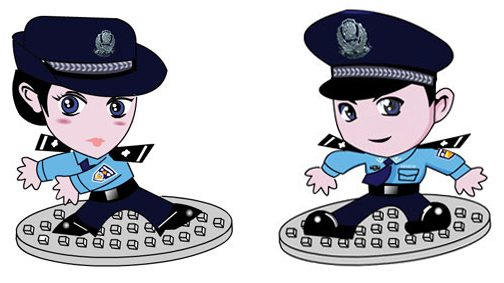
\includegraphics{figures/chap1/jingcha.jpg}
    \caption[Jingjing et Chacha, les policiers de l'Internet chinois]{Jingjing et Chacha sont deux figures créées par les autorités chinoises pour signifier la présence policière en ligne aux internautes. Le nom de ces veilleurs dessinés est une composition issue du mot “police” en chinois (jingcha). Source : \url{http://jswm.newssc.org/system/2008/10/29/011233423.shtml} consultée le 17 Février 2014, à 15:32}
    \label{fig:jingcha}
\end{figure}


Au-delà de l’activité manuelle de milliers d’employés, GFW opère également plusieurs type de blocages sur les contenus. Techniquement, la plupart du filtrage se déroule au niveau du fournisseur d’accès avec notamment des adresses particulières qui sont rendues inaccessibles : l’adresse facebook.com ou youtube.com renvoie une erreur “404 : Le site demandé n’existe pas”. Ainsi, de nombreux sites célèbres ne sont pas accessibles (Twitter, Youtube, Facebook, etc.) Les autres blocages effectifs s’effectuent selon les adresses IP ou les serveurs d’attribution de noms de domaine (DNS) menant parfois au blocage de serveurs entiers \cite{Winter2012}. Les URLs des pages de certains sites importants sont également filtrées. Sur Wikipedia notamment, la page “Tiananmen Square protests of 1989” est inaccessible depuis la Chine sans que le site Wikipedia soit pour autant intégralement bloqué. Également, des requêtes contenant des mots “interdits” sur les moteurs de recherche peuvent conduire à des micro-coupures ou un accès restreint au web pendant parfois plusieurs minutes5. La liste des sites et mots bloqués n’est pas publiée par le gouvernement et l’ajout sur ses listes s’effectue a priori sur la demande de différentes agences gouvernementales chinoises, sans notification publique. Essentiellement, il s’agit de sites à caractère pornographique (la pornographie est illégale en Chine), de sites liés aux groupes dissidents chinois (Falung Gong, Dalai Lama, Tibet Libre...), de sites du gouvernement taiwanais et d’autres sites revendiquant la liberté d’expression pour la Chine6.

Si le GFW est un outil de contrôle politique, il participe également largement au protectorat économique chinois. L’expansion rapide du vaste marché de l'Internet en Chine s’est faite sous un strict contrôle politique et si l’État a largement financé les infrastructures, GFW a été l’un des moteurs de la croissance des grandes sociétés du web chinois. L'absence du géant YouTube a notamment permis aux acteurs locaux de la vidéo en ligne de se développer rapidement, comme Youku, aujourd’hui sujet à une valorisation colossale sur les marchés d’affaires. La situation est similaire pour les réseaux sociaux. L'absence de concurrence étrangère due à l’interdiction de Facebook en 2008 puis Twitter en 2009 a permis aux acteurs chinois de se développer. Leur poids sur le marché intérieur les autorise aujourd’hui à rivaliser avec leurs concurrents américains au niveau mondial tant en nombre d’utilisateurs \cite{CIC2012} qu’en revenus directs et indirects générés \cite{CIW2012}.

Ainsi, GFW a affecté l’économie du pays en profondeur et à ce titre notamment continue d’être une préoccupation première du pouvoir politique. L’évolution technologique de GFW suit de près l’évolution des moyens de contournement des blocages, qui sont nombreux. Ainsi, le célèbre logiciel Tor garantissant l’anonymat sur Internet est aujourd’hui bloqué en Chine \cite{Winter2012} ainsi que d’autres technologies communes d’anonymisation (comme le proxy notamment). Pourtant, il reste très facile de “faire le mur” (fanqiang) et d’accéder aux contenus en contournant les limites du GFW. Les solutions techniques à disposition sont multiples et souvent peu couteuses à mettre en place ou à utiliser. De nombreux services commerciaux proposent de se connecter depuis d’autres pays à l’aide d’un VPN (Virtual Private Network) pour un coût très faible. Le VPN permet de se connecter depuis une machine située dans un autre pays et de bénéficier ainsi de l’accès tel qu’il existe dans le pays où se situe la machine. Le flou juridique qui entoure l’existence de services commerciaux de contournement de GFW témoigne de l’intérêt du gouvernement chinois à protéger largement le marché intérieur en supprimant l’accès aux services majoritaires du web occidental, sans pour autant exercer une traque systématique de chaque personne voulant utiliser Facebook ou Gmail. De plus, l’absence totale de moyens de contournement interdirait l’accès à des sources précieuses d’informations professionnelles (notamment Twitter) et se ferai donc au prix d’une perte d’avantages concurrentiels décisifs pour les entreprises chinoises, que les autorités chinoises ne semblent pas désirer. Une étude de l’OpenITP parue en 2013 analyse l’usage des outils de contournement de la censure auprès d’un échantillon de 1175 utilisateurs en Chine. Au-delà des solutions technologiques variées, on peut noter que la première raison pour contourner le blocage de l’Internet et l’utilisation des services de Google (notamment de Gmail, dont le débit est très lent depuis la Chine), suivi de la volonté de se rendre sur les sites des réseaux sociaux américains comme Facebook et Twitter, puis de l’accès aux contenus d’actualité, de vidéo en ligne et de matériel à caractère pornographique. Les utilisateurs souhaitant accéder à des contenus à caractère politique ou utilisant l’Internet de manière anonyme pour communiquer de façon plus sécurisée représente moins de 10\% de la population étudiée \cite{OpenITP2013}. Il est également important de noter que l’immense majorité des internautes chinois n’utilisent pas de système de contournement des blocages de l’Internet. 

\section[Médias sociaux en Chine : un paysage morcelé]{Médias sociaux en Chine : un paysage morcelé}
Alors qu’un blocage officiel s’applique donc sur les plus célèbres services Internet américains, de nombreux services se sont développés pour répondre aux besoins et intérêts des internautes chinois. Cette situation particulière influe sur les contenus diffusés et les usages possibles du réseau par ses membres. Au-delà des caractéristiques politiques et économiques du web chinois, d’autres phénomènes liés à ce développement technologique particulier viennent influencer la culture des entreprises web et l’être-ensemble des usagers en ligne. Dans la seconde partie de ce chapitre, nous allons présenter les différents services de réseaux sociaux en ligne (Social Network Services : SNS) les plus utilisés en Chine. Nous nous attarderons sur le cas de Sina Weibo qui sera utilisé comme support pour la suite de la présente étude. 

Profitant de l’absence des grands noms du réseau social en ligne, de nombreux services ont vu le jour sur la Toile chinoise. L'importance du guanxi \cite{Yu2008}, élément profond de la culture traditionnelle poussant chaque Chinois à entretenir et exposer avec soin ses relations en société, peut également avoir contribué à créer un terrain idéal pour le développement rapide de ces sites \cite{Arbor2011}. Plutôt morcelé, le paysage des SNS en Chine offre une variété de services et d’acteurs qui rassemble les internautes chinois selon leurs centres d'intérêts. Douban offre aux jeunes « branchés » de partager lectures, films et musique. Kaixin001, plus centré sur les jeux, propose un espace ludique pour les trentenaires au bureau. Renren (anciennement Xiaonei) est, quant à lui, un véritable clone de Facebook et se focalise sur le monde étudiant chinois \cite{Renaud2011}. Malgré ces nombreux concurrents, le service de messagerie instantanée QQ reste le leader incontesté du marché chinois. Aujourd’hui classé 8ème site le plus visité au monde7, QQ dénombre jusqu’à 100 millions d’utilisateurs connectés simultanément8. Considéré comme la quatrième plus grande firme du web mondiale, son créateur le géant Tencent Holdings Limited a investi depuis le début de l’Internet en Chine dans de nombreux domaines des TIC : jeux, publicité en ligne, e-commerce, etc. Plus qu’une simple messagerie de chat, les services de QQ sont multiples : la page de profil de chaque utilisateur (QZone) permet de maintenir un blog et d’écouter de la musique (QQmusic). Chaque utilisateur peut se créer un avatar en ligne pouvant recevoir de nombreux vêtements et accessoires vendus en ligne (QQshow) mais aussi participer à de nombreux jeux multi-joueurs pour tous les âges (QQ Entertainement). Le système de monnaie virtuelle (QCoin) mis en place pour les achats en ligne a généré dès son lancement en 2005 un nombre important de transactions9, poussant Tencent à obtenir une licence bancaire. L’utilisation de la messagerie QQ, réseau social avant l’heure, est devenu un véritable phénomène de société porté par la diversification de Tencent dans de multiples secteurs sous une marque unique. Au-delà des jeunes et des professionnels de l’Internet, le réseau QQ comptait en juillet 2011 plus de 812,3 millions de comptes actifs, faisant de lui le deuxième réseau social mondial après Facebook. Du magasin de photocopie de quartier au réseau de prostitution clandestin, QQ héberge les discussions quotidiennes et fait pour ainsi dire partie intégrante du paysage des villes modernes. Les chinois échangent plus volontiers leurs numéros de QQ que ceux de leurs téléphones portables et ce mode de communication est souvent préféré au mail dans les échanges au bureau. Convergeant rapidement avec la croissance fulgurante du e-commerce en Chine, les produits dérivés estampillés QQ sont devenu une véritable mode en Chine : voitures, téléphones, boissons, etc. Le groupe Tencent poursuit son évolution avec le lancement en 2008 de son service de microblog Tencent Weibo, qui a connu un véritable succès dès les premiers mois. Aujourd’hui, la firme de Shenzhen poursuit la conversion de ces utilisateurs QQ vers sa plateforme mobile WeChat qui connait actuellement une très forte croissance, au point de voir les autres services de microblog mis au banc par les utilisateurs. A l’origine application de messagerie écrite et vocale, Tencent continue de se diversifier en offrant désormais d’utiliser son compte QQ comme moyen de paiements pour de nombreux services du quotidien (taxis, nourritures, etc.)10.

\subsection[Microblog en Chine et Sina Weibo]{Microblog en Chine et Sina Weibo}
Les sites de microblogging (en chinois weibo) permettent aux utilisateurs de poster de courts messages composé de photos ou de texte de 140 caractères maximum, puis de les commenter et de les partager avec leurs lecteurs. A l’image de Twitter, chaque utilisateur peut souscrire aux fils d’info d’autres utilisateurs afin de recevoir leurs messages et mises à jour.

L’histoire du microblog en Chine débute en 2007 avec plusieurs services se présentant alors comme des clones de Twitter. Le service Fanfou connait notamment un succès rapide alors que de nombreux journalistes l’utilisent pour enquêter et coordonner leurs actions lors de l’arrivée du SRAS ou le tremblement de terre de Wenchuan dans le Sichuan en 2008. Le service qui connaît un rapide succès est fermé sur ordre du gouvernement en juillet 2009, suite aux nombreux commentaires suscités par des émeutes s’étant déroulé à Urumqi dans la province du Xinjiang. A peine un mois après cette fermeture, la firme SINA Corporation saisit l’opportunité et s’installe en lançant son propre service de microblog intitulé Sina Weibo. Sina Weibo connaît une croissante soutenue avec plus de 10 millions de nouveaux inscrits par mois et devient en 2012 la plateforme de microblog la plus utilisée en Chine avec 250 millions d’utilisateurs \cite{Milhard2012}. Les revenus de Sina Weibo ne cessent alors de croître (+19\% en 201211) alors que plus de 86 millions de messages sont postés chaque jour sur ce service12. 


\begin{figure}[h]
    \centering
    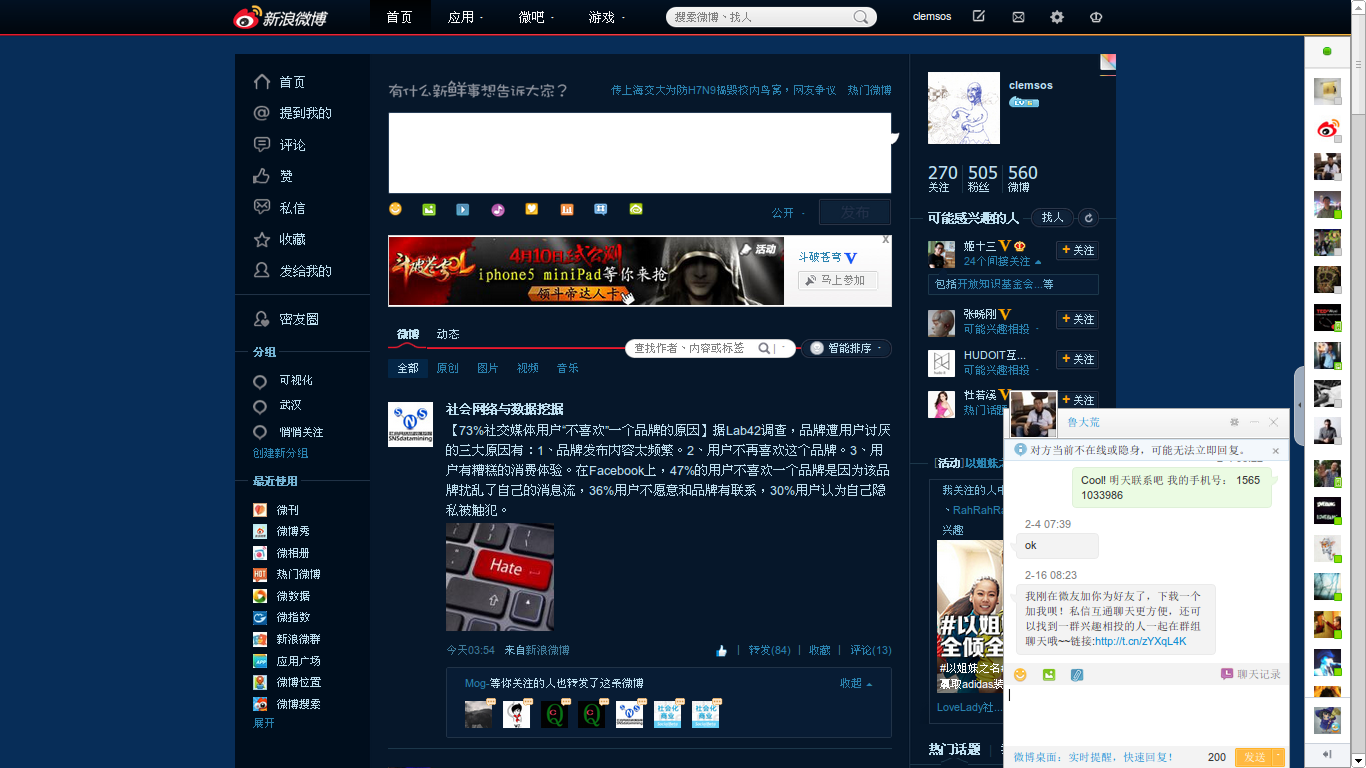
\includegraphics[scale=0.3]{figures/chap1/screenshot.png}
    \caption[Capture d’écran de Sina Weibo]{Capture d’écran de Sina Weibo, réalisé le 9 Avril 2013 à 08:59}
    \label{fig:screenshot_weibo}
\end{figure}


Figure historique de l’Internet chinois, SINA Corporation est célèbre pour son portail sina.net et son immense plateforme de blogs qui en font le fleuron des fournisseurs de contenus en ligne en Chine. Spécialisé dans “l’infotainment” (un mélange très tabloïd d’actualité et de news people), SINA est la première compagnie nationale chinoise a avoir été listée au NASDAQ dès Avril 2000. Avec son Weibo, la firme réussit un coup de force commercial et prouve une fois encore combien la censure gouvernementale est bénéfique à l’industrie du web chinois. Néanmoins, la réussite de SINA et de son service de microblog ne se fait pas sans connaître de nombreux ajustements parfois chaotiques. En effet, la stratégie agressive d’acquisition d’utilisateurs qui pousse la croissance Sina Weibo se fait avec la garantie pour les utilisateurs de pouvoir discuter et s’informer plus facilement en ligne. Dès le début de l’année 2010, les suppressions de comptes utilisateurs et de messages non désirés commencent à se répandre dans le service. Les discussions politiques sont régulièrement effacés et Sina se voit contraint de mettre en place un système de censure efficace sous la pression du gouvernement de Pékin. Néanmoins, afin de continuer à garantir la croissance du service, la firme de Pékin laisse une relative liberté aux utilisateurs en étant plutôt large sur la surveillance des discussions et les actions prises. Des personnalités publiques ou journalistes devenues “weibo-stars” mobilisent régulièrement l’opinion publique autour des sujets d’actualité attirant souvent des millions de lecteurs et de commentaires. Plusieurs scandales éclatent en ligne, mettant en cause des officiels et leur famille13. Le 23 Juillet 2011, deux trains déraillent sur la ligne reliant Ningbo à Wenzhou qui venait d’être inaugurée en fanfare quelques jours auparavant, faisant près de 40 morts et 200 blessés. La colère gronde alors que le gouvernement tarde pendant plusieurs jours à prendre la parole sur ce sujet d’actualité épineux. Sur la toile et Sina Weibo en particulier, les discussions vont bon train et les internautes indignés commentent le dernier drame du développement trop rapide de la Chine, où se mêle détournement d’argent public, corruption et sécurité des passagers. 


\begin{figure}[h]
    \centering
    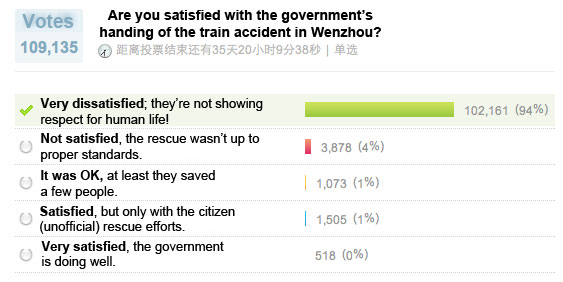
\includegraphics[scale=0.7]{figures/chap1/train.jpg}
    \caption[Sondage Weibo concernant l'accident de train de Wenzhou]{Un sondage publié sur Sina Weibo (traduction C. Custer, Tech in Asia, 1er Aout 2011), consulté le 24 Février 2014, à 22h12.}
    \label{fig:poll_weibo}
\end{figure}

Sina Weibo désactive alors la fonction de commentaires des messages. Dans les jours qui suivent, le gouvernement fait enfin une déclaration officielle sur les causes de l’accident de train puis se décide à agir en mettant en garde les internautes trop audacieux de représailles à venir. Les messages controversés sont supprimés, plusieurs comptes utilisateurs sont fermés, la police convoque les meneurs des discussions et d’autres mesures d’intimidation sont menés auprès des journalistes et des stars du weibo qui se seraient exprimés un peu trop directement à l’égard du Parti. Dans le même temps, le gouvernement a du mal à se saisir de ce nouvel outil. Alors que les administrations locales, universités et les médias d’État ont plutôt bien réussi le virage de leur stratégie de communication vers le microblog, les membres du gouvernement de Pékin ouvrent des comptes où ils sont parfois raillés, tournés en ridicule et harassés de questions. En Février 2012, les quatre plus grosses sociétés de microblog (dont Sina Weibo) annoncent que chaque utilisateur est maintenant contraint de modifier son profil pour mentionner son véritable nom, prénom ainsi que son numéro de carte d’identité. Cette velléité de vérification échoue et est abandonnée quelques semaines plus tard face à la mobilisation des utilisateurs et la difficulté de faire appliquer de telles mesures. Le gouvernement de Pékin édite pourtant une série de règles \textit{“Several Regulations on Microblog Development and Administration Enacted by the Beijing Government”} dont la plus notable sera la possibilité de condamner tous ceux qui auront participé à la diffusion d’information considérées comme fausses, erronée ou mensongères. Face à la multiplication des actions gouvernementales et à l’apparition d’autres plateformes, la croissance du nombre d’utilisateurs de Sina Weibo est désormais stoppée pour aborder une phase de déclin estimé à près de 10\% dans les deux premiers mois de 201414. 

A la lecture de l’histoire de Sina Weibo on constate l’ambivalence des actions officielles du gouvernement chinois dans la réussite économique des entreprises d’Internet. Si la firme SINA a bénéficié de prime abord d’un avantage compétitif notoire par l’élimination de la concurrence, elle a par la suite souffert des conséquences du contrôle politique de l’Internet, avec notamment une perte de ses utilisateurs.

\begin{figure}[h]
    \centering
    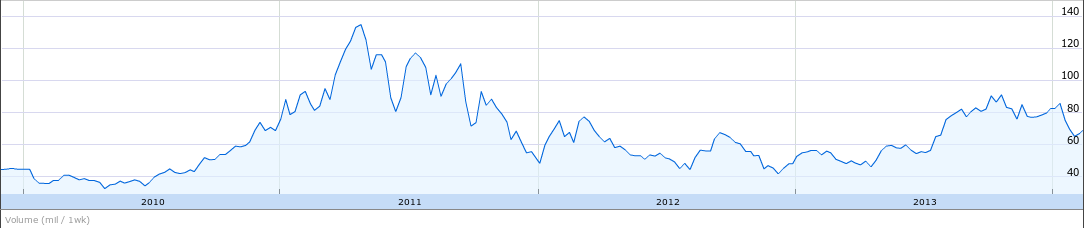
\includegraphics[scale=0.4]{figures/chap1/sina.png}
    \caption[Cours de l’action SINA au Nasdaq entre 2009 et Février 2014]{Cours de l’action SINA au Nasdaq entre 2009 et Février 2014 - Source : Google Finance, consulté le 17 Février 2014 à 15:28 }
    \label{fig:sina_nasdaq}
\end{figure}


\subsection[Sina Weibo, un usage plus ludique que Twitter ]{Sina Weibo, un usage plus ludique que Twitter }
Dans son article nommé A Tale of two microblogs, Jon L. Sullivan \cite{Sullivan2013} raconte comment l’évènement historique de la fermeture de Twitter en Chine a vu la communautés des microbloggers chinois se scinder en plusieurs groupes distincts : 
Twitter rassemble une communauté avide de libres discussions, souvent très politisée voire radicalement en opposition avec le gouvernement chinois.
Tencent Weibo est utilisé par les utilisateurs de QQ, typiquement des personnes aux revenus plus faibles qui accèdent au web depuis leurs mobiles
Sina Weibo est le favori des travailleurs urbains, souvent plus jeunes ou éduqués, représentant davantage la classe moyenne montante.

Dans la littérature en sciences informatiques, plusieurs articles propose des comparaisons entre Twitter et Sina Weibo. Une large analyse quantitative et comparative menée avec des jeux de données des deux services \cite{Qial2012} nous apprend que le contenu de Sina Weibo est davantage corrélé avec des sentiments positifs (analysés automatiquement). Les utilisateurs de Sina Weibo parlent davantage de lieux et de personnes alors que les utilisateurs actifs sur Twitter s’intéressent plus aux organisations. Également, Sina Weibo connaît un pic d’activité le week-end alors que Twitter affiche généralement une baisse de régime dans les fins de semaine. Ces différentes indications suggèrent une tendance où Sina Weibo serait davantage utilisé pour des activités de loisir quand Twitter se destinerait à un usage plus professionnel. Une étude s’intéressant aux tendances sur Sina Weibo \cite{Lial2013} indiquent que la majorité des comptes les plus influents de Twitter ont été vérifiés contrairement à Weibo où le taux est plus faible chez les grands utilisateurs. La vérification d’un compte se fait par l’authentification auprès du fournisseur de service afin d’attester la véracité de la personne utilisant le compte. C’est un enjeu important pour les figures publiques (marques, stars, homme politiques, etc.) Cet indicateur nous montre donc l’intérêt professionnel fort qui entoure Twitter, moins pressant dans le cas de Sina Weibo où moins de personnes ont ressenti la nécessité de faire officialiser leurs comptes. Sur les deux services de microblog, les utilisateurs inscrits possèdent un réseau de relations identifiables par leur souscription aux fils d’infos d’autres utilisateurs (follow). La relation peut être inexistante (none), mutuelle (friend) ou unidirectionnelle (follow : un utilisateur suit un autre mais n’est pas suivi par ce dernier). La comparaison d’échantillons des graphes sociaux issus des deux services \cite{Chenal2012} montrent comment les relations sur Sina Weibo sont plus dissymétriques et moins réciproques, reflétant une hiérarchie plus forte entre les utilisateurs que Twitter. 

Un autre facteur important de différentiation entre les deux services est la nature de la diffusion des contenus postés sur Sina Weibo. Contrairement à Twitter où le texte domine, la majorité des posts de Weibo contiennent des images ou des vidéos \cite{Zhao2012}. Les posts possédant des contenus multimédia (images, vidéos...) sont plus susceptibles d’être diffusés largement et restent en moyenne actifs pour une durée plus longue \cite{Zhao2012}. Également, les contenus sur Sina Weibo possèdent une proportion moins élevée de retweets et de commentaires que sur Twitter \cite{Zhao2012, Gao2012}. L’activité de la population de Twitter est plus intense, moins tournée vers la diffusion de masse et plus réactive aux influx de nouveaux contenus. 

Nous voyons donc que le paysage de Sina Weibo se constitue autour de stars et célébrités qui concentrent l’attention avec des contenus à la diffusion très large. Moins tournés vers l’actualité et la conversation que son homologue Twitter, Sina Weibo agit comme véhicule de contenus à grande audience, souvent publiés par des personnalités publiques célèbres. Des études quantitatives montrent bien que les contenus les plus échangés et discutés concernent les loisirs et divertissements, la mode, la santé, etc. \cite{Lial2013}. Les messages à caractère humoristique (texte, images et vidéos) occupent également une place prépondérante dans les échanges des utilisateurs, contrairement à son homologue américain Twitter dominé plutôt par les sujets d’actualité \cite{Yual2011}. Sina poursuit ainsi son rôle historique de leader dans le domaine de l’infotainment. 

Pourtant la population de jeunes urbains qui soutient la croissance de son service de microblog reflète aussi les transformations en cours dans la société chinoise. Les journalistes et spécialistes de l’information sont les premiers à se saisir de ce nouveau média. Dans un discours à Stanford en 2013, le PDG de Sina Charles Chao explique : 

\begin{quote}
“Le plus grand changement apporté par le microblog en Chine concerne d’abord l’industrie des médias elle-même. Aujourd’hui, plus de 30\% des actualités ont d’abord été reportées sur Sina Weibo avant d’atteindre les médias 	traditionnels. Le rôle des médias traditionnels a été déplacé vers un traitement des informations en profondeur (in-depth reporting).” (traduction de l’auteur)
\end{quote}

\footnote {Charles Chao, PDG de Sina pendant la Stanford Graduate School of Business China 2.0 tenue le 3 Octobre 2013. Disponible en vidéo \url{http://www.youtube.com/watch?v=tlliivJKHk8}, consultée le 19 Février 2014 à 11:23}

L’omniprésence des supports mobiles (smartphones, tablettes)16 permet en effet des modes de traitement de l’information jusqu’ici inconnus qui bousculent les hiérarchies très contrôlées des salles de rédaction chinoises. Alors que la population urbaine croît rapidement, le smartphone est “the first big urban purchase” \cite{Wallis2013} pour ceux qui arrivent en ville et représente un outil indispensable de participation à la société. En 2008, la Chine était le seul pays en Asie où les moins de 30 ans possédait plus d’amis en ligne que hors ligne \cite{Synovate2009}. Ainsi, les réseaux sociaux jouent un rôle primordial dans la socialisation urbaine et viennent changer les modes d’expression. Il est à noter que les spécificités de l’écriture chinoise rendent possible l’écriture d’un court texte en 140 caractères, alors qu’une telle longueur autorise seulement une courte phrase dans une écriture utilisant un alphabet latin. Alors que le lectorat chinois a perdu toute confiance dans la plupart des médias traditionnels suite à l’absence répétée de courage et à la rétention d’information cruciale dans les dossiers importants qui animent le pays, le microblog s’installe comme une nouvelle source de confiance pour des millions de citoyens voulant comprendre et prendre part aux changements cruciaux de la Chine moderne.

Un rapport de l’Institut de Journalisme Reuters à l’Université Oxford paru en 2013 montre comment les usages du microblog ont amené des transformations dans le quotidien des journalistes chinois. Le journalisme d’investigation a notamment connu un essor important avec le renouvellement des sources grâce à une large diffuson en ligne des sujets. Sina Weibo n’a pas amélioré nécessairement la qualité de leurs investigations, mais a par contre permis une plus grande dissémination. La mobilisation des utilisateurs pour la protection des journalistes a également joué un rôle important ainsi que le renforcement de procédés de vérification existant depuis longtemps sur les forums du web chinois. Très populaire dans les années 2000, Le \textit{“moteur de recherche de viande humaine”} (\textit{renrou sousuo}) est une forme de traque d’individu en ligne réalisée par un large nombre d’internautes à partir d’un nom ou d’une photo. Il s’agit souvent de retrouver quelqu’un désigné comme “coupable” (d’adultère, de corruption, etc) en réunissant un maximum d’informations à travers la Toile afin d’identifier ou de localiser la personne. Devant les dérapages rapides de ce type de procédés, les questions d’éthique du journalisme en ligne sont au coeur des discussions pour les journalistes et les titres de presse. En effet, l’usage des médias sociaux permis à certains journalistes de faire pression sur les pouvoirs publics, amenant parfois à la censure de leurs travaux, mais a également permis une très large auto-promotion pour de nombreux journalistes devenus des stars de weibo.

Le contrôle des contenus sur Weibo est donc une réalité quotidienne et a été depuis son lancement la source de plusieurs études. Les formes les plus courantes sont : la suppression de posts, la suppression de comptes utilisateurs et le blocage de mots-clés. Le blocage de mots-clés s’effectue dans le moteur de recherche interne du site (“pas de résultats” quand vous chercher un mot bloqué) et plus récemment par l’impossibilité de poster un message contenant des mots ou des adresses web bloqués \cite{Ng2013}. La pratique de la suppression de comptes s’est intensifiée en 2013\footnote{ \textit{“Over 100,000 Sina Weibo Accounts Shut Down or Penalized for Govt Rules Violations”} par Gabriela Vatu, 14 November 2013 \url{http://news.softpedia.com/news/Over-100-000-Sina-Weibo-Accounts-Shut-Down-or-Penalized-for-Govt-Rules-Violations-400289.shtml} consulté le 17 Février à 16:42} avec notamment la suppression de millions de “zombies” présents sur le site. Les “zombies” sont des comptes utilisateurs créés par des robots qui se chargent de reposter automatiquement des contenus, souvent afin d’augmenter le trafic sur le site. Les exigences des annonceurs publicitaires de plus en plus présents sur le site ont obligés Sina Weibo à faire la chasse aux robots sur son site, faisant ainsi diminuer le nombre de comptes actifs de manière significative. La firme Sina est garante auprès du Ministère de la Sécurité Publique chinois des contenus qu’elle diffuse et effectue à ce titre une surveillance constante pour supprimer les messages “non-conformes”. Lors de nos recherches, nous avons constaté que l’interface de Sina Weibo garde la trace des commentaires supprimés par le système d’administration. Dans les messages supprimés se trouvent à la fois des posts d’utilisateurs “zombies” et les posts jugés incorrects par les administrateurs. Au total, la suppression des messages s’effectue avec un taux estimé à environ 16\%, allant jusqu’à plus de 50\% dans certaines provinces comme Ningxia ou le Tibet contre seulement 12\% à Beijing \cite{Bamman2012}.


\begin{figure}[h]
    \centering
    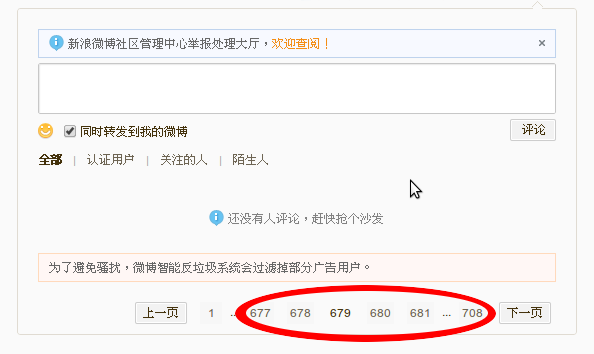
\includegraphics[scale=0.5]{figures/chap1/comments.png}
    \caption[Commentaires supprimés par Sina]{La trace des commentaires supprimés par Sina est encore visible - Page 677 à 708, les commentaires ont été supprimées, soit approximativement 4\% messages supprimés (589 messages sur 13452, à raison de 18 à 20 messages par page). Capture d’écran effectuée le 29 Janvier 2013 à 12:32:42, http://www.weibo.com/1701401324/zeoBquVKi, consulté le 16/02/2013.}
    \label{fig:comments}
\end{figure}


\section[Code, langage et milieu(x) numérique(s)]{ Code, langage et milieu(x) numérique(s)}
L’espace d’expression offert par l’Internet chinois et ses services de réseaux sociaux possède donc de multiples particularités et amène une variété de pratiques, de questions et de réflexions qui nécessitent d’être appréhendées avec des outils de problématisation et d’analyse spécifiques. Dans la troisième et dernière partie de ce chapitre introductif, nous allons donc nous pencher sur les concepts existants dans la littérature scientifique qui peuvent nous éclairer sur l’existence in situ des objets numériques. Afin de mettre en perspective le Web chinois et l’histoire de ces objets, nous introduirons notamment le concept de milieu numérique, héritier de l’idée complexe de milieu que nous explorerons ci-après.

\subsection[Lieu, espace, territoire et technologies]{Lieu, espace, territoire et technologies}
Géographie, management et diffusion de l’innovation, histoire des technologies, cultural studies ou études “nationales”, les travaux qui s’intéressent aux relations entre technologies, espace, lieux et territoires sont nombreuses et offrent un paysage riche où se croisent de nombreuses disciplines scientifiques. L’influence des réseaux de transports sur l’expérience humaine et le développement des villes a notamment été largement étudiée \cite{Offner1993,Doulet2001}. L’Internet lui-même a également fait l’objet de nombreuses études monographique (par pays) ou comparative, une étude à l’échelle mondiale présentant en effet des problèmes de données et évidemment d’échelle \cite{Dupuy2004}. En Chine où l'urbanisation produit actuellement une vaste mobilité notamment des ruraux qui arrivent en ville, l'utilisation des réseaux sociaux médiatise bien souvent les choix de lieux et les rencontres des nouveaux arrivants. De nombreux groupes de discussions réunissent par exemple les nouveaux acheteurs d’immobilier qui échangent leurs stratégies d’achat et de défenses de leurs droits et de leurs biens, organisant aussi des rencontres \cite{Li2013}. L’usage des réseaux sociaux revêt pour les nouveaux arrivants une importance capitale, notamment dans la recherche de groupes similaires et l’échange d’expériences. La disponibilité des données et le rôle croissant de la cartographie dans l’usage d’Internet viennent produire un « Geoweb » constitué de données et métadonnées spatiales \cite{Crampton2009}. Les vastes quantités de données produites par les multiples humains et machines sont souvent réunies et comprises dans leur attachement commun à un lieu physique \cite{Torrens2010} offrant un point d'entrée unique (Open Data territorial, geo-localisation, GIS, POI\footnote{GIS : Geographic Information System ; POI : Point-Of-Interest}, etc.) par le marqueur spatial du geotag \cite{Reference}.

La carte notamment a joué sur le web un rôle important d’abord en tant qu’illustration, puis plus récemment d’interface avec le réel. Loin d’être figé par le territoire, la carte le décrit sous un ou des angles particuliers \cite{Brunet1987, Jacob1992}. Le développement de standards comme le système GPS \cite{Haklay2008} et de services et outils de cartographie ont contribué a une appropriation de la pratique cartographique par un nombre croissant de personnes \cite{Crampton2008}. De nouvelles formes de données produites par les utilisateurs parfois appelées \textit{« volunteered geographic information »} \cite{Elwood2008} utilisent les services en ligne comme Google Maps pour dessiner un « miroir du monde offline » \cite{Graham2011}. Le courant dit de la néogéographie utilise abondamment le GIS et les outils en ligne (Google Maps, Flickr, etc.) pour comprendre les pratiques de ces nouvelles formes de \textit{« géographies volontaires »} \cite{Turner2006}. Cette présence accrue dans le réseau dessine l’enjeu non seulement de cartographier le monde, mais également de cartographier le réseau lui-même, ouvrant ainsi de nouvelles voies pour découvrir la construction sociale des espaces par des pratiques individuelles et de groupe. Dans cette étude, nous avons donc choisi d’interroger les objets numériques afin de comprendre comment se structurent la parole et la conversation dans le contexte unique de l’Internet chinois. Afin d’articuler les multiples dimensions d’analyse qui viennent enrichir notre réflexion, il nous faut donc brosser un portrait en large de l’Internet chinois, en le considérant tour à tour comme un espace structurant pour les actions des internautes qui le pratiquent, comme un territoire sujet aux relations de pouvoir actualisées par les groupes et individus et enfin comme un lieu habité par ceux qui y construisent chaque jour des significations communes. Nous proposons donc ici une revue sélective des quelques travaux à même de nous apporter des éclairages pertinents dans la vaste littérature s’intéressant aux dimensions géographiques des TIC.

\subsubsection[Code / space : l’espace transductif des TIC]{Code / space : l’espace transductif des TIC}

Dans leurs recherches autour de la géographie des technologies numériques, Dodge  Kitchin ont travaillé à développer le concept de code comme un élément fondateur des espaces modernes dans lesquels nous évoluons. Reflétant l’importance croissante accordée aux TIC dans l’environnement urbain, ils citent un travail sur la production automatique des espaces : \textit{“De plus en plus, les espaces de la vie  quotidienne nous parviennent chargés de logiciels (software)”} \cite{Thrift2002} En effet, si le projet urbain a été guidé pendant le demi-siècle dernier par l’apparition de la technologie automobile dans l’espace des rues, les TIC paraissent prendre le relais avec l’idée d’une ville intelligente et connectée, connue sous le nom de \textit{« smart cities »} \cite{Ascher2009}. Dodge \& Kitchin ont donc fait du code une des pierres d’angles de l’appréhension de l’espace dans leur travail en le définissant comme suit : 

\begin{quote}
« an instruction or rule that has a single outcome determined by a binary logic (yes/no). The combination of these indidivuals logic rules produces code (program)” \cite{Kitchin2011}.
\end{quote}

La part croissante des TIC dans nos espaces quotidiens amènent les auteurs à envisager l’espace dans son interaction avec le code, symbolisant la suite d’instructions machiniques et électroniques qui permettent à un espace de remplir sa fonction. Dans un article intitulé \textit{Flying through code/space: the real virtuality of air travel}, Dodge \& Kitchin analyse la structure des espaces aéroportuaires. De l’achat des tickets jusqu’au vol des avions en passant par la gestion des bagages, le bon fonctionnement d’un aéroport est entièrement conditionné par le bon fonctionnement des longues successions d’instructions du code. Ici, Dodge et Kitchin propose le concept de code/space pour décrire ce type d’espace spécifique où lorsque le code échoue (failure) alors le code/space tout entier échoue \cite{Dodge2004}. L’exemple de l’aéroport est parlant : si le système de check-in des bagages ou les machines responsables du contrôle de sécurité des passagers ne fonctionnent pas, alors l’espace aéroportuaire ne peut exister en tant qu’aéroport. L’analyse de la spatialité ne se situe alors plus dans un domaine sémantique ou narratif, mais plutôt dans les processus et opérations qui s’y déroulent et le code et les technologies y jouent un rôle primordial : 

\begin{quote}
« Code is employed as the solution to a problem, a particular kind of transduction 	is occurring.» \cite{Kitchin2011}. 
\end{quote}

L’espace n’est pas un donné mais s’explique plutôt comme : \textit{“une forme d’ontogénèse (en perpétuel devenir-au-monde), l’espace est une pratique; un faire ; un évènement (…) qui ne pré-existe pas à son faire (doing)”}. L’espace est considéré non pas comme une production, mais comme une transduction. Reprenant le travail de Simondon sur l’individuation par la technologie, Dodge  Kitchin présente l’espace comme une pratique qui comprend les actes, actions, occurrences, mémoires, perceptions, etc. d’un groupe d’individus s’y trouvant. La fonction de l’espace structure et est structurée par les individus et le code y est considéré comme une entité agissante. Dans le code/space, la relation dyadique entre code et espace est bijective: l’un ne peut aller sans l’autre. En terme simondonnien, la \textit{transduction} ne peut être assurée sans code. Si l’exemple de l’aéroport illustre bien cette nécessité du code dans le devenir-espace, Dodge  Kitchin ont également identifié d’autres catégories où cette relation est plus ténue : les \textit{coded spaces}, qui peuvent poursuivre leurs fonctions même lorsque le code échoue ; les \textit{background coded spaces} où les processus de transduction induit par l’espace ne s’appuie pas nécessairement sur le code, mais propose néanmoins des possibilités de l’activer (machine éteintes ou inactives, etc.) 

L’analyse fonctionnelle des rapports entre espace et technologie de Dodge  Kitchin offre à voir comment les TIC peuvent être un facteur \textit{transductif} pour les individus se mouvant dans les espaces de leurs vies quotidiennes. Si nous appuyons pleinement ce constat, il nous semble que le parti-pris des auteurs de considérer le “code” comme une abstraction incluant uniquement les instructions ou “logiques machiniques“ ferme la porte à l’immense densité des activités symboliques qui se jouent dans l’usage des technologies. Comment notamment considérer les “contenus” du web dans cette grille de lecture? Comment resituer dans une perspective historique les logiques de médiation de l’espace par les technologies de l’écriture? Il nous semble en effet que la faillite fonctionnelle (\textit{failure}) des code/spaces précède l’arrivée des technologies et s’opère déjà à un niveau symbolique - la fonction de l’espace du Palais du Louvre après la chute des rois de France se voit radicalement modifiée. La transduction opéré lors de la pratique d’un espace s’effectue donc dans un jeu d’appropriation symbolique qui passe notamment mais pas seulement par les technologies. Ici les technologies du langage et de l’information jouent notamment un rôle crucial dans l’affirmation du récit symbolique (\textit{narrative}) qui construit l’espace. L’activité du code dans la structuration des code/space de Dodge  Kitchin existe donc sous une forme non seulement fonctionnelle mais également sémantique, voire phatique ou même esthétique comme l’a décrit Jakobson dans ces analyses des fonctions du langage \cite{Jakobson1956}. Au-delà de sa dimension machinique, le code possède les caractéristiques d’une poiesis dépassant l’idée simple de fonctionnalité pour exister dans la complexité d’une écriture comme traduction du langage humain et machine.

\subsubsection[Codes, discours et territoires des technologies]{Codes, discours et territoires des technologies}

Le code serait davantage à comprendre comme un mode d’expression humain à travers la technologie, actualisant l’\textit{episteme} décrit par Foucault dans \textit{Les Mots et Les Choses} comme l’élément fondamental de la pensée d’une époque et sa considération pour le monde \cite{Foucault1996}. Définie comme l’état des connaissances scientifiques et littéraires, l’episteme existe comme la somme des savoirs d’une époque présupposée traduite en un regard sur le monde. Le \textit{code} exprimé dans de nombreux langages est une écriture où s’expriment les savoirs d’aujourd’hui. Le code source d’une page Internet, d’un programme informatique ou d’un driver hardware ne s’écrit pas seulement en langage “machine” mais mélange langages informatique et humain. A la fois production savante, outil scientifique, vecteur d’expression et interfaces des savoirs, le code constitue l’expérience narrative du monde par les TIC. Possédant de nombreux mots, aspects et syntaxes issus de multiples langues humaines, les replis de l’écriture informatique laisse transparaitre de tout bord leur origine humaine. Les standards d’encodage des bases de données comme l’Unicode deviennent presque le nouvel alphabet de notre écriture \cite{Guichard2014}. Une minorité de personnes savantes, “lettrés” de l’informatique déchiffrent et écrivent le code alors que l’immense majorité se voit frappée d’illettrisme devant l’arrêt soudain de l’ordinateur ou la perte d’un fichier. Ainsi, la définition du “code” de Dodge  Kitchin doit être étendue pour recouvrir plus largement les pratiques symboliques liés aux activités de l’écriture du code dans ces espaces.

Le code ainsi redéfinit nous ramène alors à une lecture foucaldienne du discours dans sa relation intime avec le territoire \cite{Foucault2004}. Dans ces nombreux travaux sur la généalogie, Michel Foucault cherche à comprendre comment les relations de pouvoir créées par les discours portés sur les objets préside à la production de territoires, d’interdits comme autant de sujets de ces discours. Nous définissons la \textit{discursivité} comme le processus de construction de ces discours, et ce faisant le processus de définition des territoires de l’Internet issus de la pratique du code. Historiquement, l’Internet a été très tôt sujet à l’appropriation par le discours de nombreux groupes actifs dans leur volonté de territorialisation. La métaphore géographique et spatiale a structuré le vocabulaire de l’Internet dès sa création \cite{Graham1998} : \textit{site}, cyberspace, etc. L’\textit{Electronic Frontier Foundation} se charge de protéger l’u-topie qu’est Internet avec JP Barlow qui rédige la fameuse \textit{Déclaration d’Indépendance du Cyberespace} \cite{Barlow2001}. A l’opposé du spectre, les autoroutes de l’information in-forment le paysage comme autant de géogrammes massifs \cite{Berque1999}. L’appropriation des protocoles du réseau, la lutte pour la défense de standards ouverts sont autant d’expression qui s’ancrent dans les pratiques du discours, dont les mots free et open cristallisent l’histoire de luttes de revendication des territoires de l’Internet \cite{Blondeau2000}. L’autre grande métaphore constitutive de l’Internet est textuelle avec ses pages, langages et hypertextes \cite{Vandendorpe1999}. La formule choc \textit{« Code is law »} \cite{Lessig2009} résume l’idée  que les processus textuels du code mettent en jeu un ensemble de rôles, protocoles et mises en scène qui agissent comme autant d’autorités à travers le discours. La jurisprudence fait loi comme écrit sur les murs des bureaux de Facebook à Palo-Alto : \textit{« Code wins arguments »} \footnote{Dans la Lettres aux Investisseurs écrite par M. Zuckerberg  pour l’IPO de Facebook \url{http://www.sec.gov/Archives/edgar/data/1326801/000119312512034517/d287954ds1.htm\#toc287954_10}}. La territorialisation de l’Internet se fait donc au travers d’un ensemble de pratiques discursives, méta-grammaire des discours en ligne où les luttes symboliques se jouent dans les pratiques discursives du code. La confrontation symbolique au sein des territoires numériques se poursuit dans le discours, réifié dans les pratiques du code. Les structures fonctionnelles et symboliques deviennent les stratégies de production de territoires qui se définissent dans l’usage des langages. 

Sur l’Internet chinois, les pratiques de censure de l’écriture en sont le reflet le plus frappant. Blocage de mots-clés, détournements de langage, suppression et modification de texte sont l’expression de cet affrontement de discursivités parfois antagonistes. La Grande Muraille gouvernementale scanne les masses de texte pour reconnaître et stopper des mots tels que \textit{« Printemps arabe »} ou \textit{« évènements de Tian-An Men »} \cite{McKinnon2009}. Néanmoins, l’état actuel des techniques de \textit{data mining} ne permet pas encore de déceler les phénomènes langagiers comme les jeux de mots ou l’ironie. Bien souvent, les internautes chinois choisissent l’humour pour permettre à leurs idées de se frayer un espace. Revêtant leurs masques de chat, les internautes chinois sont devenus spécialistes dans la publication de jeux de mots, chansonnettes et petites vidéos d’animaux, comme autant de couperets cinglants pour railler les officiels trop pompeux de Pékin. Dans la guerre de l’information que se livrent sans cesse censeurs et internautes, les véritables héros sont bien souvent de simples photos truquées de crabes et de lamas. Ces blagues numériques, d’apparence bien souvent inoffensive, font chaque jour le tour de la Toile chinoise, portant en elles toute la subversion d’internautes aspirant à plus de liberté. Début 2010, alors que pleuvaient les longs discours pieux du Parti sur l’harmonie de la nouvelle société (en chinois \textit{hexie}), on voit apparaître en ligne des essaims de crabes de rivière (se prononçant également \textit{hexie}) couverts de chaînes en or criant : \textit{“Vive l’harmonie”} au volant de leur limousine. Devenus aujourd’hui une image vivante de la corruption des hauts dignitaires du Parti, on croise régulièrement dans les commentaires d’un article officiel un petit crabe de rivière, comme un petit rappel posté par un lecteur.


\begin{figure}[htp]
    \centering
    \subfloat[]{\label{fig:hexie-meme}
\includegraphics[scale=0.5]{figures/chap1/hexie.jpg} 
    \hspace{5pt}
    
    \subfloat[Discours du PCC sur l’harmonie]{ \zh{和谐} (hexie) : Harmonie}
    \hspace{5pt}

    \subfloat[Mèmes / humour des internautes]{ \zh{河蟹} (hexie) : Crabe de rivère}}
    \hspace{5pt}


    \caption[Hexie]{ Mot de la semaine : Crabe de Rivière - China Digital Times du 21 Mars 2012 - Licence Creative Commons http://chinadigitaltimes.net/2012/03/word-of-the-week-river-crab/, consulté le 15 Février 2013.}

    \label{fig:hexie}
\end{figure}



On voit bien comment le code décrit ici un territoire sujet à l’autorité politique sous la forme d’un système de \textit{data mining} cherchant à mettre en forme le discours. La fonction du \textit{code/space} sémantique que forme ici l’espace de l’Internet est réécrit par un jeu de langage et la circulation d’objets digitaux permet de reterritorialiser cet espace en apparence régit par un code strict de censure. 

\subsubsection{Les lieux des technologies comme }
Dans son célèbre livre sur les Arts de Faire, De Certeau \cite{DeCerteau1980} considère la ville comme un texte dont chaque piéton énonce et révèle (\textit{performe}) des sens nouveaux par son activité de marcheur. Actualisant l’espace urbain par sa marche, l’habitant de la ville s’approprie des lieux qui restent néanmoins partagés avec d’autres. Au détour des rues, le sens commun des lieux urbains se construit avec les multiples énonciations de ceux qui les habitent et les font vivre. Cette magnifique image de la poésie du texte urbain met en lumière la dualité que nous avons abordé précédemment avec la \textit{transduction} de Simondon : l’espace ne peut fonctionner sans les pratiques de ceux qui l’habitent. Plus encore, l’être-ensemble et le devenir-soi procèdent de la construction de lieux communs, \textit{poiesis} des espaces habités. Les TIC font aujourd’hui souvent partie intégrante des lieux que nous habitons. Graham \cite{Graham1998} dans son travail sur l’étude des lieux et de leur rapport à la technologie identifie trois types majeurs d’approches dans la littérature :


\begin{enumerate}

\item L’approche \textit{« substitutive »} ou \textit{« transductive »} qui voit dans l’arrivée des TIC la disparition de la valeur des lieux, dans un idéal de proximité utopique \cite{McLuhan1962} ou un discours dystopique sur leur proche disparition \cite{Virilio1998, Augé1995}. Ces considérations sont les formes traditionnelles du débat accompagnant l’innovation dont sont férus la communication industrielle et la critique des médias \cite{Ramonet2001}, restant souvent purement prospectif et faisant peu de cas des usages.

\item Plus modérée, l’approche qualifiée par Graham de \textit{« co-évolutionniste »} s’interroge sur la façon dont les les interactions dynamiques des espaces virtuels \textit{space of flows} et réels \textit{space of places} \cite{Castells2009} produisent de nouveaux lieux . Ces études économiques et sociales prennent la forme d’une médiologie de l’espace adaptée aux études stratégiques pour l’urbanisme et l’implantation des télécommunications. Son inteprétation par les aménageurs lui donne parfois une dimension déterministe peu utile à la compréhension des phénomènes liés à l’appropriation et l’historicité des technologies \cite{Offner1993}.

\item Une dernière approche plus récente se cristallise autour de l’idée de relations et de réseaux. Afin d’éviter l’écueil des causalités directes et de la notion fataliste d’”impact”, les lieux comme \textit{« des moments articulés dans un réseau de sens et de relation sociales »} \cite{Massey1993}, des assemblages entre objets matériels “actants” \cite{Latour1996}, individus et groupes sociaux. Cette approche s’intéresse davantage au lieu comme une géométrie sociale en mouvement, liée au temps et à la situation \cite{Thrift2001} et refuse l’idée d’une existence “virtuelle” qui serait commune à différents objets \cite{Bingham1996}.

\end{enumerate}

En privilégiant une approche dynamique et relationnelle des lieux comme constructions sociales de sens \cite{Kyle2007}, la technologie perd son rôle déterministe de productrice d’espaces et d’usages pour devenir une actualisation d’un espace-temps géographique et historique par des groupes d’individus. Comme le note Cresswell dans son travail sur les lieux : \textit{“places are practiced. People do things in place.”} \cite{Cresswell2004}. Il propose trois aspects pour décrire l’actualisation des lieux par leurs pratiques : location (un point dans l’espace, \textit{“the ‘where’ of place”}), \textit{locale} (les aspects visibles et tangibles du lieu, \textit{“the way a place looks”}) et \textit{sense} (\textit{“the feelings and emotions a place evokes”}). Néanmoins, cette définition ne permet d’appréhender l’existence des lieux en ligne (le site web d’un lieu est-t-il une \textit{locale} ou une partie du \textit{sense}?). Graham et Zook propose le concept de DigiPlace afin de décrire plus spécifiquement l’existence des lieux en ligne : \textit{« DigiPlace - that is, the use of information ranked and mapped in cyberspace to navigate and understand physical places (…) In other words, DigiPlace represents the simultaneous interaction with software (information) and `hard-where' (place) by an individual.»} \cite{Zook2007}. S’inspirant des travaux de Harley sur le pouvoir du cartographe, leur travail sur le rôle de Google Maps dans la présence des lieux sur Internet met à jour l’interaction et l’hybridation entre existence spatiale et existence en ligne constituant des DigiPlace. 

Les phénomènes de transduction à l’œuvre dans les pratiques spatiales de l’Internet sont donc le reflet des états du réseau à un moment donné, les lieux eux-mêmes formant ainsi un réseau basé sur leurs relations et similarités. Brunet dans son \textit{Vocabulaire de la Géographie} propose notamment l’idée de synapses : \textit{«espaces ou lieux par lesquels on passe, par où l'on communique, les isthmes, les détroits, les estuaires, les carrefours, les ports et les ponts, etc.; »} \cite{Brunet1993}. Envisagés par leur fonction “synaptique” , les lieux deviennent alors un construit social au rôle clair, évitant l’écueil d’une qualification en-soi. Aéroports, hypermarchés, aires d’autoroutes ou zones industrielles ont été qualifiés de \textit{non-lieux} par Marc Augé, produits d’une  hyper-modernité \textit{« qui ne peut se définir ni comme identitaire, ni comme relationnel, ni comme historique. »} \cite{Augé1995}. Réfuté plus tard par l’auteur lui-même, cette idée de lieux simplement \textit{produits}, et non construits fait l’impasse sur la tension d’usage, le devenir lieu que modèlent ses utilisateurs assidus ou épisodiques, ceux qui y travaillent voire même y habitent. Le lieu n’est pas nécessairement “patrimonial” comme produit d’une histoire, mais peut \textit{« être ou ne pas être un non-lieu selon le statut de l'individu envisagé. »} \cite{Debarbieux1993}. Les hypermarchés et leurs galeries marchandes sont des haut-lieux de socialisation et de rencontres pour les adolescents qui vivent en banlieue \cite{Matthews2000} mais paraissent froids et inhumains aux habitants des rues du centre-ville.

L’étude menée par Puel, Pons et Xiaoting autour des pratiques sociales environnantes les café Starbucks de Beijng (Chine) montre également comment la stratégie marketing de la firme s’appuie précisément sur cette “absence patrimoniale” pour faire sa place au travers du vaste territoire chinois. La non-existence d’un \textit{“bon café avec Internet”} dans les villes chinoises offre la possibilité aux clients, usagers de ces cafés récemment apparus de s’y rendre pour utiliser l’Internet ou retrouver leurs amis \cite{Puel2007}. Ainsi, l’absence d’histoire n’interdit pas de la constitution de pratiques communes à forte valeur symbolique, qui sont à comprendre ici dans des réseaux d’appartenances mondiaux (jeune, dynamique, urbain, etc.). Dans son livre \textit{The Great, Good Place}, Ray Olenburg propose le concept de tiers-lieu pour décrire ces lieux qui, séparés de l’environnement de travail ou de la maison, permettent de se socialiser. Jouant un rôle majeur dans la construction de communautés et la constitution d’une société civile, ces tiers-lieu doivent répondre à certains critères comme : un coût d’accès nul ou modeste, une très bon accessibilité, la présence régulières des \textit{« habitués »}, un lieu acceuillant et confortable et enfin un lieu où l’on peut rencontrer facilement de nouvelles personnes \cite{Oldenburg1999}. L’idée de tiers-lieu virtuels a également été mentionnée pour désigner les chatrooms ou les plateformes de réseaux sociaux en ligne qui rempliraient des fonctions sociales similaires \cite{Soukup2006}. 

Nous voyons donc qu’en considérent les lieux de l’Internet, nous mettons à jour un ensemble de pratiques qui ne s’intéresse plus nécessairement à l’ordre du discours (et aux pratiques de censure notamment) mais plutôt aux phénomènes d’individuation, notamment au travers des multiples actes d’énonciation qui forment les pratiques et usages du web. Dans cette étude nous cherchons donc à comprendre de manière plus profonde comment les internautes habitent leur Internet. Il ne s’agit pas d’analyser le discours en terme de relations de pouvoir mais plutôt d’essayer de distinguer comment les circulations des objets numériques sont structurantes pour les pratiques des internautes, comme autant de lieux habités quotidiennement.

\subsection[Le milieu : richesse et désuétude ]{Le milieu : richesse et désuétude }
Afin de problématiser les relations entre protocoles du discours et pratiques locales d’appropriation, nous avons choisir d’introduire le concept de \textit{milieu numérique}. Nous définirons d’abord brièvement ce concept avant de présenter un regard historique sur l’idée de milieu dans les sciences. Nous discuterons ensuite de l’acception particulière que nous avons choisi de défendre ici et nous verrons comment cette notion sera utile pour la suite de notre étude sur les réseaux sociaux en Chine.

\begin{quote}
L’idée de milieu numérique est a priori définit dans les termes suivants : 
“The multiple networks, which are connected by protocols and standards, constitute what I call a digital milieu.” \cite{Hui2012}
\end{quote}

L’usage de multiples interfaces et le dédale des réseaux TIC constitue \textit{“un nouveau milieu perceptif”} \cite{Weissberg2007}. Notre milieu physique est aujourd’hui (déc)ouvert par l’existence de notre milieu digital qui nous aiguille: rencontres, restaurants, voyages, etc. sont bien souvent médiatisés par l’Internet en premier lieu. Ainsi, nous évoluons dans un milieu numérique qui agit comme support des processus de transduction et de connaissance du monde. Le code prend ici pleinement part à la construction de ce milieu digital, à la fois déterminant pour la production des actes de discours et ouvert à l’appropriation des pratiques et usages du quotidien.

Historiquement, le concept de milieu se détache du centre pour resituer et mettre en perspective la relation des êtres à leurs environnements sous des jours parfois contradictoires. Débattue puis écartée mais toujours très usitée, la notion de milieu introduit autant le déterminisme d’un combat pour la survie et l’adaptation, que la liberté créatrice du sujet dans un univers ouvert à sa volonté. 

Pour illustrer au mieux l’extraordinaire fécondité philosophique de la notion de milieu, nous allons tout d’abord essayer de comprendre la trajectoire de ce mot durant les siècles derniers \cite{Canguilhem1965}. Sans pour autant remonter à son aube étymologique, nous nous apercevons que le mot milieu décrit un trajet singulier dans le monde des sciences. Employé dès le 16e siècle par Descartes dans son Traité de la lumière, il représente pour Newton une mesure de distance dans l’éther, cette non-matière qui structure la gravitation et fait se mouvoir les objets. Défini plus tard par d'Alembert dans son encyclopédie comme un : \textit{"espace naturel dans lequel un corps est placé, qu'il se meuve ou non"}, le mot connaitra durant tout le XIXème un large développement sémantique en s'étendant de la physique à la biologie. Les naturalistes français de l’époque affirme que le milieu n’est pas seulement \textit{environnant} mais influe sur les êtres vivants. Ainsi Lamarck dès 1809 écrira dans sa \textit{Philosophie Zoologique}: \textit{"le milieu a une grande puissance pour modifier les organes"}. Par la suite dans l’histoire du XXème siècle, nous pouvons identifier deux moments marquants pour ce concept et structurants pour l’histoire des sciences dans son ensemble \cite{Taylan2010}. 
Le premier se joue sous la plume d’Auguste Comte qui, inspiré de la biologie naissante, articule le vital au social dans la sociologie naissante et décrit le milieu comme \textit{« l’ensemble des circonstances extérieures (…) nécessaires à l’existence de chaque organisme déterminé »} \cite{Comte1838}. Sans sombrer pour autant dans un déterminisme total, Comte introduit une première dialectique des rapports avec le milieu comme conditions de possibilité de la vie : \textit{« Tout être vivant (…) modifie sans cesse son milieu. »}, écrit-t-il alors. 
Le concept qui connait un succès croissant en France est peu de temps après réapproprié par les penseurs d’Outre-Rhin qui lui donnent alors un sens différent. S’opposant au francisé \textit{Der Milieu}, le géographe Ratzel introduit dans son \textit{Anthropogéographie} (1899) le mot \textit{Umwelt} qui se démarque rapidement par sa dimension fortement déterministe. Dans un même mouvement, le physiologue et biologiste Jakob von Uexküll étudie dans son laboratoire la tique et se rend compte que le milieu de la tique se définit non pas par tout l’environnement qui l’entoure mais seulement par ce qui lui est utile et approprié. Le milieu devenu \textit{Umwelt} s’oppose alors à l’environnement indifférencié et devient l’ensemble des éléments qui sont porteurs de significations (\textit{Merkmalträger}) pour un être. 
Uexküll propose ainsi une \textit{« biologie subjective »} qui étudierait les relations de chaque espèce avec son milieu. Dans l’Allemagne du siècle débutant, Uexküll cherche à diffuser largement sa théorie qui s’adresse pas tant aux animaux qu’à l’humain dont le milieu serai la Patrie (\textit{Heimat}) \cite{Feuerhahn2009}. Reflétant les débats guerriers entre la \textit{Kultur} allemande et la \textit{Civilisation} française \cite{Elias1975}, se cristallise dans l’idée de Milieu une tension politique sur les relations entre nature et vivant qui devra déchirer l’Europe pendant longtemps encore. Foucault dans son cours au Collège de France du 11 Janvier 1978 parle de l’influence de l’idée de milieu sur la conception du territoire pour les urbanistes du XVIIIème siècle. Quand sous Louis XIV, les villes étaient construites d’après un espace conçu comme vide (voir \textit{Richelieu} en Indre-et-Loire), la question de l’urbaniste du XVIIIème est de comprendre la ville dans son évolution future. L’enjeu est devenu l’\textit{adaptation} du milieu existant (à la fois urbain et naturel), la transformation du \textit{donné} compris comme un élément qu’on peut venir modifier. L’idée sous-jacente de milieu ouvre la possibilité de l’appropriation de la nature. En terme foucaldien, cette nouvelle bio-politique se fonde sur la territorialisation du milieu comme nouveau centre des enjeux de pouvoir. L’ère industrielle réalise ce projet d’une adaptation à la fois \textit{au} et \textit{du} milieu vu comme tension nécessaire de l’évolution, passage obligé vers la civilisation. Alors que l’humain s’est vu déplacé dans son rôle central par l’astronomie galiléenne puis l’évolution darwinienne, l’idée de milieu pose comme enjeu majeur du vivant la maitrise de l’environnement - la lutte pour ne pas être maitrisé. Poursuivi par la psychanalyse de Freud qui introduit l’Autre au sein du sujet, l’entreprise de décentrement de l’humain vers son milieu se joue dès l’abord dans les termes de la vie ou de la mort. Plus tard, Lacan identifiera la transition de la petite enfance à l’enfance par le « stade du miroir » comme moment où l’enfant différencie enfin le Milieu (Umwelt) du Soi (InnenWelt) \cite{Lacan2001}. Ce "passage au milieu" est donc d’une importance capitale puisque s’y joue la constitution de l’être.

L’approche du milieu comme élément unificateur des sciences est également un sujet toujours en discussion. L’écologie notamment a largement recentré le milieu sur le rôle déterminant de l’Homme par l’introduction du concept d’\textit{environnement} \cite{Gandalfo2008}. Les conséquences de ce passage de l’idée de nature à celle de milieu restent profondes, notamment dans le droit civil où nous sommes passés d’un rapport du « droit imposé » de la nature au « droit négocié » du milieu \cite{Papaux2008}. Méta-réflexion, la discussion sur le "milieu académique" donne lieu à d’intéressants échanges \cite{Stengers2009} qui interrogent notamment la définition trop abrupte des disciplines scientifiques et leur herméticité. Parfois nommé \textit{mésologie}, l’étude du milieu se donne pour mission de réconcilier des pratiques diverses de la biologie à la sociologie en imaginant une étude par le milieu \cite{Stengers2003}. Les œuvres de Deleuze  Guattari, dont la mésologie se revendique, parlait déjà de la pratique d’une philosophie du milieu : \textit{"Partir au milieu, par le milieu, entrer, sortir, non pas commencer ni finir, […] renverser l'ontologie, destituer le fondement, annuler fin et commencement.[…] C'est que le milieu n'est pas du tout une moyenne, c'est au contraire l'endroit où les choses prennent de la vitesse."} \cite{Deleuze1972} 
La réflexion sur la technique et les technologies s’est notamment saisie à bras le corps de cette notion, avec notamment l’idée de \textit{milieu technique} par Friedman et Leroi-Grouhan \cite{Stiegler1998}. Tout geste (du plus banal au plus rare) s’effectuerait dans un milieu technique qui le rend possible. Gilbert Simondon dans son livre Du mode d’existence des objets techniques continue cette réflexion avec ce qu’il appelle le milieu associé : 
\begin{quote}
« médiateur de la relation entre les éléments techniques fabriqués et les éléments 	naturels au sein desquels fonctionne l’être technique. (...) C’est ce milieu associé 	qui est la condition d’existence de l’objet technique inventé. » \cite{Simondon1989}. 
\end{quote}
Simondon problématise le milieu associé comme vecteur de l’\textit{individuation}, où se produit la rencontre entre objets et individus pour chacun les actualiser. Poursuivant ce travail, Stiegler comprend les technologies de l’information comme un milieu essentiellement social, comprenant à la fois ce qui est autour de l’individu (environnement) et entre les individus (medium) \cite{Reference}. Sans sa lecture critique des industries culturelles, Stiegler formule l’idée qu’un milieu est \textit{associatif} s’il permet l’individuation. A l’inverse, certains milieux seraient \textit{dissociatifs} car ils ne permettraient pas le devenir individu, à l’image des mass media qui divisent producteurs et consommateurs de symboles. La dynamique industrielle des deux derniers siècles a entraîné une massification des phénomènes culturels, créant un milieu technique considéré comme largement dissociatif car dé-réalisant les individualités \cite{Simondon1989}. Néanmoins, le renouveau technologique porté par l’apparition des technologies numériques ouvre aujourd’hui une page nouvelle pour l’individuation en offrant un milieu extrêmement associatif, fondé pour ainsi dire sur le lien. Voyant un nouvelle âge des Lumières \cite{Stiegler2012}, Stiegler conçoit l’Internet comme un milieu qui ne serait pas structurellement dissociatif et pourraient donc recréer de nouvelles formes plus horizontales d’économie symbolique où existent davantage de symboles partagés. 

\subsection[Cyberespace et milieu numérique]{Cyberespace et milieu numérique}
Associateur ou dissociateur, les protocoles qui régissent l’accès au milieu sont donc les enjeux politiques du milieu numérique, conditionnant l’existence des objets numériques. L’étude des relations entre espace et dispositifs socio-techniques ne se comprend donc pas seulement en termes d’infrastructures, mais plus finement dans l’observation et la description d’une géographie du réseau. Les débuts de la géographie au XIXème siècle définisse en effet cette discipline comme la science des milieux. Vidal de la Blanche cherche alors à expliquer comment les actions humaines sont déterminés par des faits “naturels” pré-existants. Alors que la sociologie fait école, les géographes aux aussi commencent à considèrer les œuvres humaines comme partie intégrante du ou des milieux qui les produisent \cite{Demangeon1942}. Cette nouvelle géographie humaine cherche à inclure à mettre en relation : \textit{“l'étude des relations verticales qui se développent au sein de chaque milieu, et celle des relations horizontales qui mettent en relation les milieux”} \cite{Claval1990}. Les réflexions géographiques sont nourris par de vastes controverses sur de nouveaux paradigmes : l'espace, le territoire, le paysage, les lieux qui estompent peu à peu l’idée déterministe de milieu pour développer un appareil conceptuel plus complexe. Le développement méthodologique avec notamment la géomatique et les outils d’analyses issu de la statistique permettent de proposer des lectures variés de faits géographiques divers. Brunet définit les \textit{chorèmes} comme des \textit{“structures élémentaires d'organisation de l'espace”} \cite{Brunet1980}, Berque parle de géogrames définis comme \textit{"motif éco-techno-symbolique (...) au sein de la relation qu'est l'écoumène"} \cite{Berque1999}. Inspiré de la philosophie japonaise moderne, l’écoumène de Berque se rapproche de l’idée de milieu et est décrit comme une vaste matrice relationnelle des choses et des êtres - une dimension écologique générale, une \textit{“trajectivité”} \cite{Watsuji2011}. Au sein de cet écoumène, le géograme offre un modèle des faits géographiques où se rejoignent les aspects techniques, symboliques et sociaux (les relations humaines). Alors que la notion de milieu disparait peu à peu pour être remplacée par celle d’environnement\cite{dAngio2001}, l’espace des géographes se voit bientôt augmenté d’une nouvelle réalité à prendre en compte: le cyberespace. Espaces, sites, routes, les nombreuses métaphores géographiques viennent remettre en question des pans enteir de la discipline et renouveler les approches. Le cyberespace, \textit{“hallucination consensuelle”} décrite par Gibson \cite{Gibson1984} déclare bientôt son indépendance \cite{Barlow1990} et dessine ainsi une géographie virtuelle \cite{Batty1997} qui s’interroge sur les dimensions de ces nouveaux espaces décrits par la circulation d’information. Les structures spatiales et économiques préexistantes semblent être renforcées par les stratégies territoriales et les équipements des acteurs. L’importance des Etats-Unis \cite{Zook2001, Cukier1999} dans la localisation des flux Internet (capital, data centers, noms de domaines...) montre bien comment les évolutions technologiques participent à la fragmentation territoriale à l’échelle du mondiale. Néanmoins, les routes de l’Internet s’écartent aussi bien souvent des autoroutes de l’information pour venir construire des sens beaucoup plus locaux par les nombreux mécanismes des activités en ligne. \textit{“cyberspace is ‘made real’ through the language of place”}, comme l’écrivent justement Dodge \& Kitchin \cite{Dodge2007}.
S’opposant aux objets naturels et techniques, les objets numériques sont à comprendre dans leurs relations matérielles et temporelles avec les infrastructures de leur production et archivage dans les mémoires des données du web. Ainsi, le milieu numérique dans lequel chacun évolue se présente sous la forme d’objets numériques actualisés qui fondent le milieu associé. À l’instar des des géogrames du paysage de Berque ou des chorèmes de l’espace de Brunet, nous pouvons imaginer ici des \textit{“topogrammes”} qui permettront de considérer les faits et objets digitaux. Le milieu numérique, tenant à la fois du cyber-espace (le lieu physique où se situent les machines) et constitués des objets digitaux qui lui sont spécifiquement associés. Le topograme en tant que modèle permet de décrire et considérer sous un jour commun des objets digitaux dissemblables.

Afin d’observer et de décrire le milieu numérique en Chine et de tester l’hypothèse méthodologique proposé par le notion de topogrames, nous avons choisi d’étudier de façon empirique les dynamiques à l’œuvre dans et autour de certains objets numériques particuliers sur les réseaux sociaux : les mèmes Internet. 
